\chapter{Architecture}
\label{chap:Arch}

This chapter explains the architecture of the Alternative Spaces project. The following definition of software architecture is used for this project, originally used in the book ``Software Architecture in Practice'' by \cite{bass2012software} and also used by the course TDT4240 Software Architecture at NTNU. 
\bigskip
\hfill\begin{minipage}{\dimexpr\textwidth-1cm}
\emph{"The software architecture of a program or computing system is the structure or structures of the system, which comprise software elements, the externally visible properties of those elements, and the relationships among them."}
\end{minipage}

\paragraph{} This chapter discusses the different architectural drivers, architectural views, architectural patterns, and architectural rationale of the system. The purpose of the architecture document is to supply the stakeholders with an organized description of the system architecture, to be used as a means to understand the system and as a basis for further development of the system. 

\newpage
\section{Architectural Drivers}
\label{sec:ArchDrivers}

The architectural drivers of this project are the functional requirements, quality attributes, business requirements and technical requirements. The main architectural drivers of the entire project is the non-functional requirement Usability and the functional requirements. 

\subsection{Functional Requirements}
\label{subsec:ArchDriversFunctional}
The functional requirements defines the functions of the system and its components, and the functional requirements related to this project are defined in the Requirements-document found in \ref{part:PlanReq} of the report. Because this project is a prototype, which aims at giving the customer a look into how a future system like this would work, the functional requirements are the main drivers of the architecture and have the greatest influence on the architecture of the system.

\subsection{Non-functional Requirements}
\label{subsec:ArchDriversNonfunctional}
The non-functional requirements defined for this system are usability, performance, security, availability and scalability. Of these, the the architecture mainly reflects Usability, focusing on making the web application intuitive and easy to use for the future end users. Most importantly, the system must be easily understood for a potential future pursuit of funding by the customer for a complete system. Because our product is a prototype of the future system described in the Further Work section, it is unnecessary to lay resources in creating a prototype focused on scalability, performance and security as there will be no real end users for the prototype.

\subsection{Business Requirements}
\label{subsec:ArchDriversBusiness}
The project spans over a time of 12 weeks. This is a very short period of time compared to the complexity of the product, and therefore the main business requirement of the product is to create a partial, but well-functioning prototype of the desired product for the customer within the time frame. The main influence of the business requirements in regards to the system architecture is the level of complexity and optimization of the architecture. Using complex and advanced patterns that may be more beneficial to implement than going for a head on implementation will, because of lack of experience, require too much time for research and implementation. For this reason, implementing architectural and design patterns have not been prioritized. Though the customer is the most relevant stakeholder relative to the project team in regards to the development of the system, they have little influence on the architecture of the product. The customer has expressed that technical decisions are mainly to be decided by the development team, but have still been included in every step of the process to ensure customer satisfaction.

\subsection{Technical Requirements}
\label{subsec:ArchDriversTechnical}
The technical requirements of the project include the frameworks, browsers and devices necessary to use the website and mobile application. These do not have direct influence on the architecture of the system. 


%%%%%%%%%%%%
\section{Architectural Views}
\label{sec:ArchViews}

This section describes the system from the viewpoint of different stakeholders. The four views are the logical view, development view, process view and the physical view. 


\subsection{Logical View}
\label{subsec:ArchViewsLogical}
Our logical view shows our three-tier client-server architecture tiers: the presentation tier, logic tier and the data tier. The logic tiers of both the website and the Android application are pretty much the same, except that the mobile application supports less functionality than the website. The logic view presented below represents the three tiers with examples from the sign-up process. The mobile application is limited only to sign in and sign out function and the uploading of pictures and specifying locations to these pictures.

\begin{figure}
\centering
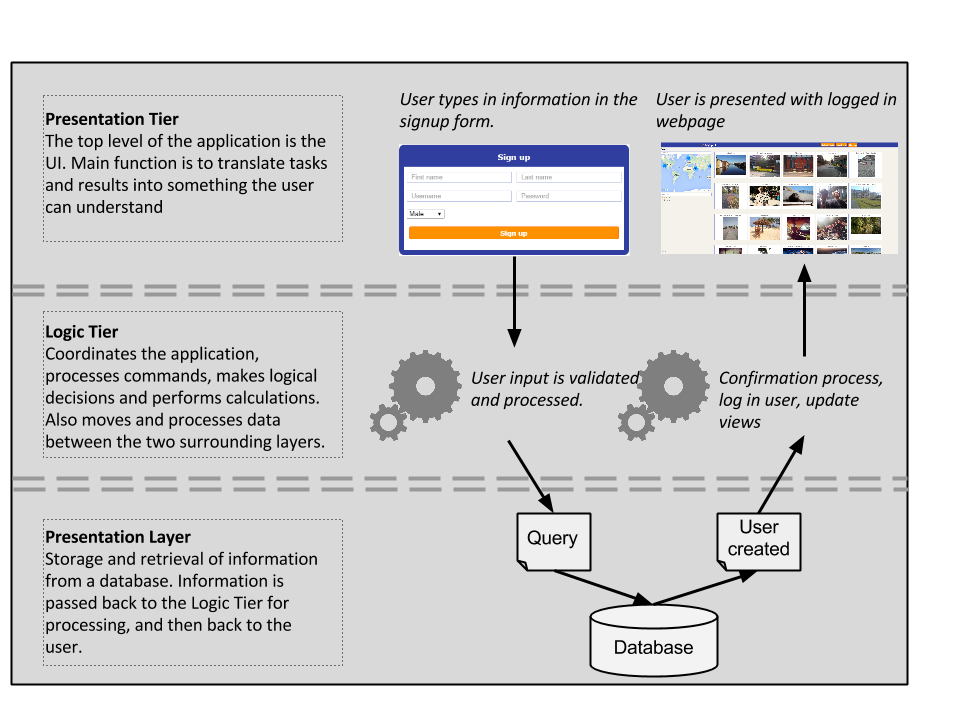
\includegraphics[width=\linewidth]{./Architecture/img/LogicView.png}
\caption{Logic View, with tiers briefly explained. \label{overflow}}
\end{figure}

\subsubsection{Presentation Tier}
The top-level tier is the information the user is presented with and interacts with on the website. The users view the content, received as HTML or JSON responses from the server, on a web browser or a mobile application, respectively.  In other words the presentation tier is the views of the web page or mobile application which the user interacts with. As the user interacts with the content of the web page or application, HTTPS/HTML calls are made to the server, which are processed and the results of the other tiers' processes are displayed to the browser/mobile application.

\subsubsection{Business Logic \& Communication Tier}
The logical tier is the layer that deals with the communication between the tiers, and the application functionality by processing the input and output information communicated between the presentation and data tier. Each client communicates directly to the server, which processes the data. The slight difference in communication on the web and mobile front it that the web clients make HTTPS/HTML (HyperText Transfer Protocol Secure) calls and responses, while the mobile clients make HTTPS calls but receive JSON (JavaScript Object Notation) responses. The logic tier is stored on the server. 

\subsubsection{Data Tier}
The data tier includes the server, with the database and the stored objects and files. The data tier receives SQL queries from the logic tier which are then processed. The data tier also stores all images and videos submitted and shared amongst users, as well as other objects used as graphics on the website. 

%\newpage
\subsection{Physical View}
\label{subsec:ArchViewsPhysical}
The physical view explains the mappings of the components that comprise the system, including server, web browsers, mobile platform, the database and the models. The physical components of the system are the server, and the clients web (e.g. computers) and mobile devices (running Android OS). All application logic is found on the server, which the clients devices communicate with.

\begin{figure}
\centering
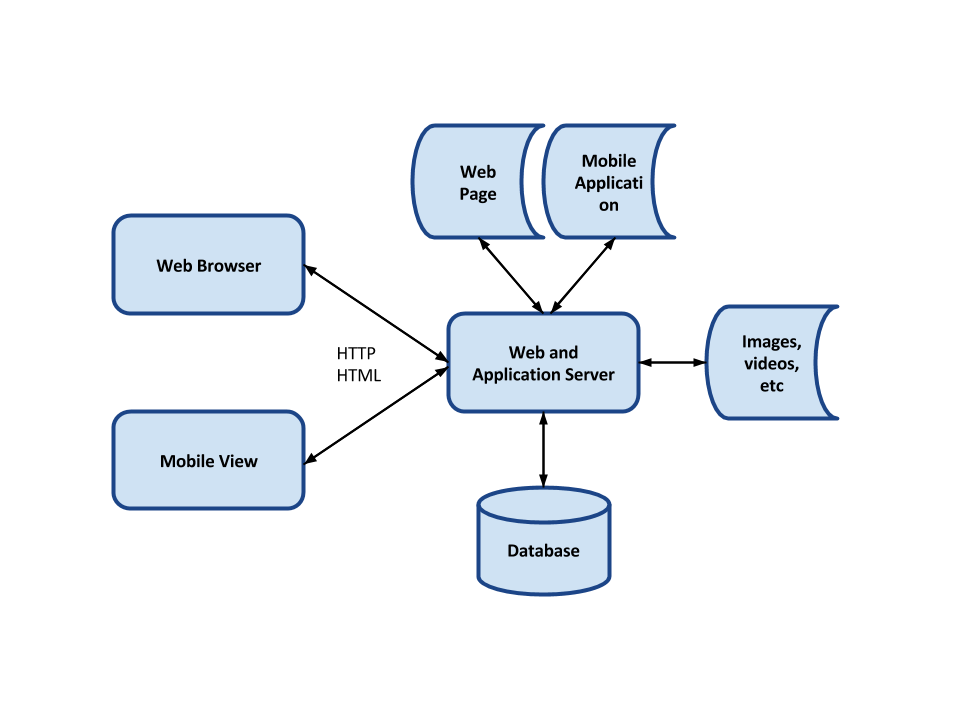
\includegraphics[width=\linewidth]{./Architecture/img/PhysicalView.png}
\caption{The Physical View of the web application. \label{overflow}}
\end{figure}

%\newpage
\subsection{Development View}
\label{subsec:ArchViewsDevelopment}
The development view shows the structure of the web application system from the developers view point. The system is divided into four different folders. Back end includes all PHP-code that has to deal with the database and web pages. The image and css folders contain graphics including all styling and images. The js folder contains all JavaScript files dealing with the interactivity between components and objects of the website. The development view for the Android application has not been included as the functions are limited, and all functions are already found on the web application.

\begin{figure}
\centering
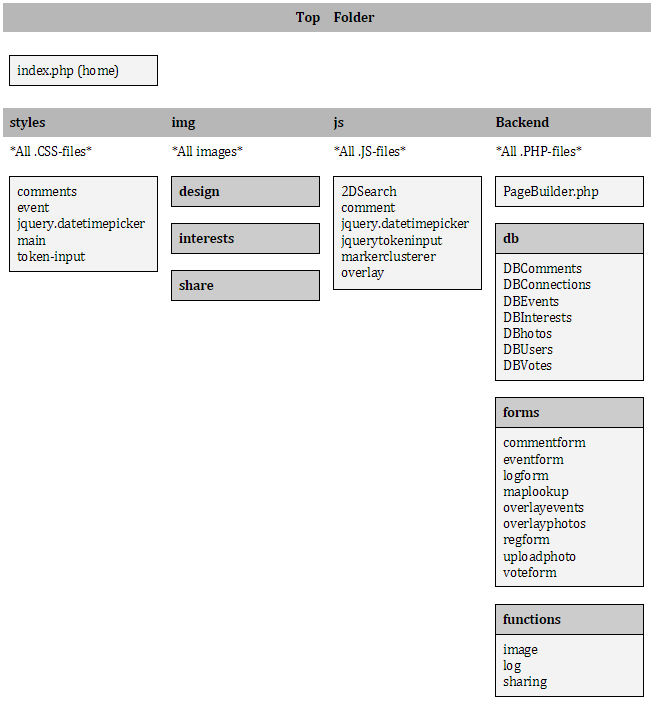
\includegraphics[width=\linewidth]{./Architecture/img/DevelopmentView.png}
\caption{The Development View of the web application. \label{overflow}}
\end{figure}

\subsection{Process View}
\label{subsec:ArchViewsProcess}
The process view is an activity diagram which shows the flow between different actions available to the user upon entering the site. Note that this is only a simplified diagram of the web application, but gives a quick overview of what actions are available to the user at different stages of the website. 

\begin{figure}
\centering
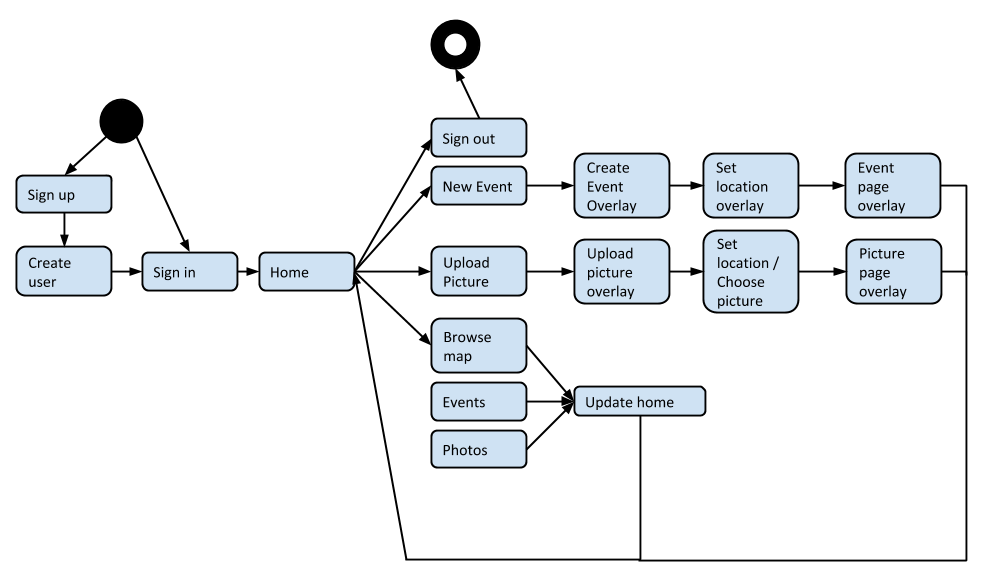
\includegraphics[width=\linewidth]{./Architecture/img/ProcessView.png}
\caption{The Process View in the form of an activity diagram of the web application. \label{overflow}}
\end{figure}


%%%%%%%%%%%%
%\newpage
\section{Architectural Patterns}
\label{sec:ArchPatterns}
The following definition of architectural patterns is used for this project, and developed by \cite{taylor2009software}.
\bigskip
\emph{"An architectural pattern is a named collection of architectural design decisions that are applicable to a recurring design problem, parametrized to account for different software development contexts in which that problem appears."}

\paragraph{} For the development of the web application four different architectural principles were merged together in during the implementation of the product. Service-oriented Architecture, Client-Server Architecture, Multi-Tier Architecture and Model-View-Controller Design Pattern were used for the web application. For the mobile application with limited functionality, simplicity was in focus. Architectures implemented on the mobile front was Client-Server, and the Model-View-Controller and Three Tier architectures as they walk hand in hand and are necessary for the mobile application to work. 

\subsection{Client-Server Architecture} 
The most obvious architecture implemented for MySplot is the Client-Server architecture. The client-server architecture is based on the principle of having one or more application servers providing a service to the clients, the end users of MySplot. As the MySplot server is connected to the internet, the service is provided for any person (client) using a web browser connected to the internet.

\subsection{Service-Oriented Architecture}
Closely tied to the Client-Server architecture is the Service-Oriented Architecture (SOA). The SOA architecture of MySplot on the web application front provides application functionality as a service to the end users' web browsers via a protocol. The service provided by MySplot is the application functionality found on the server. The development of the entire product has been implemented by actively communicating with and focusing on how the target users of the service want the final product to be. To fulfill the Client-Server and Service-Oriented architectures the Model-View-Controller and the Multi-Tier architectures have also been merged into the architecture.

\begin{figure}
\centering
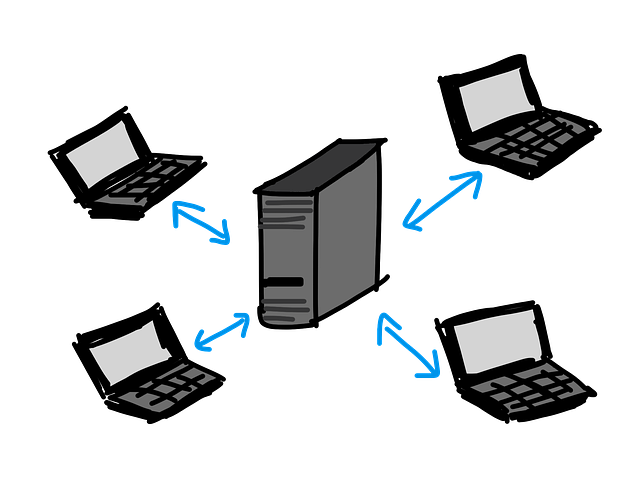
\includegraphics[width=90mm]{./Architecture/img/clientserver2.png}
\caption{Visual example of the Client-Server Architecture. \label{overflow}}
\end{figure}

%\newpage
\subsection{Three-Tier Architecture and Model-View-Controller Pattern} Three-Tier Architecture is simplest case of the Multi-Tier Architectural Pattern, including a Presentation Tier, Business Logic Tier and a Data Tier. This architectural style was introduced earlier and shown in practice in the Architectural Views section. The Three-Tier architecture deployed in MySplot has adopted the Model-View-Controller Design Pattern, whereas the controllers and views are in the presentation tier, and the model in the business tier. See the Architectural View section ``Logical View'' for a further description.

\begin{figure}
\centering
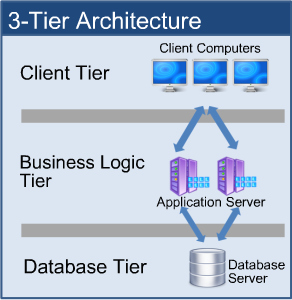
\includegraphics[width=90mm]{./Architecture/img/threetier.jpg}
\caption{Visual example of the Client-Server Architecture. \label{overflow}}
\end{figure}


%%%%%%%%%%%%
%\newpage
\section{Architectural Rationale}
\label{sec:ArchRationale}
Since the product is a website, the team chose to implement a Client-Server Architectural Pattern as it is the most widely used pattern for creating web applications to date. As the website is going to hold vast amounts of data, the introduction of a server communicating the content to the client devices significantly reduces the stress each of the client devices would have to deal with if having to store all the websites contents individually. 

\paragraph{} Furthermore, the architecture is service oriented and has been divided into three tiers, the presentation, business logic, and data tiers, to improve organization and structure in the product. These choices make it easier for the developers to have a complete overview of a system constantly expanding in size during implementation as well as making the process of modifying the system a much simpler task. The introduction of the Model-View-Controller design pattern to the three-tier architecture also supports organization and structure of the system, by clearly defining which parts handle logic and which parts handle views. Implementing the architectural patterns to the system has been a immense help on the development side. Developers can in a simple and structured way be assigned tasks that regard different aspects of the system, with the corresponding tasks being easily being created or located, and developed or modified, because of the architectural patterns. 
